\documentclass{article}
\usepackage[utf8]{inputenc}

\title{CTA200 Assignment 2}
\author{Simon Smith}
\date{May 2020}

\usepackage{natbib}
\usepackage{graphicx}
\usepackage{caption}
\usepackage{subcaption}
\usepackage{indentfirst}
\usepackage{float}
\usepackage{listings}
\usepackage{amsmath}
\usepackage{geometry}
\usepackage{url}
\usepackage{textcomp}
\usepackage{titling}
\usepackage{dirtytalk}
\usepackage{gensymb}

\geometry{margin=0.7in}
\setlength{\parskip}{1em}
\setlength{\parindent}{3em}

\begin{document}

\maketitle

\section{Q1. Behaviour of the Complex Plane}

\subsection{Methods}

It is completely nonsensical to talk about negative numbers as outputs of a squaring function for the reals, but the complex numbers, as their name may suggest, behave in curious ways. We explore the tendencies of complex numbers when iterated squaring is applied.

\begin{equation}
    z_{i+1} = |z_i|^2 + c
\end{equation}

c is some complex number of the form $a + bi$ and we take z$_0$ to be zero. Starting here, we iterate over this expression until we can determine whether the series will run off to infinity. To do so, for a given c, we let this iteration run 10 times and then examine the value of the last term. If this term is greater than 100, we know it has run far away from the origin and will continue to do so. We now run this process for every point in the complex plane ranging from (-2, 2) and (-2i, 2i) and keep track of which points stay bounded to a finite number. We plot this subset to get a curious image which has come to be known as the Mandelbrot set.

We can rewrite the code to investigate this set of complex numbers further. Some points diverge faster than others and we can keep track of how quickly each point runs off to infinity. This produces the figure on the right of Figure \ref{fig:B0353+52}, showing finer details around the edges of the set.

\subsection{Analysis}

Any number that is positive real will diverge. It seems the region of complex numbers whose absolute value is less than unity will stay bounded. If you zoom in on regions of the image, it will resemble the structure of other parts of the image.

\begin{figure*}[ht]
    \centering
    \captionsetup{justification=centering}
    \begin{subfigure}[t]{0.4\linewidth}
        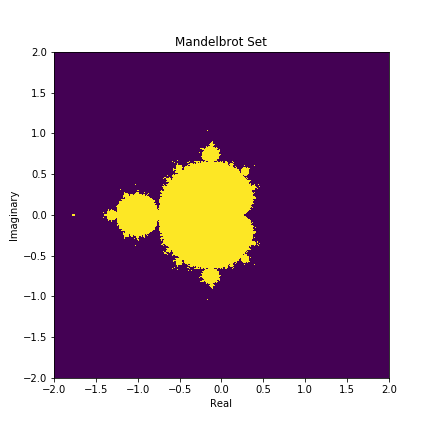
\includegraphics[width=\linewidth]{images/mandel.png}
    \end{subfigure}
    \begin{subfigure}[t]{0.535\linewidth}
        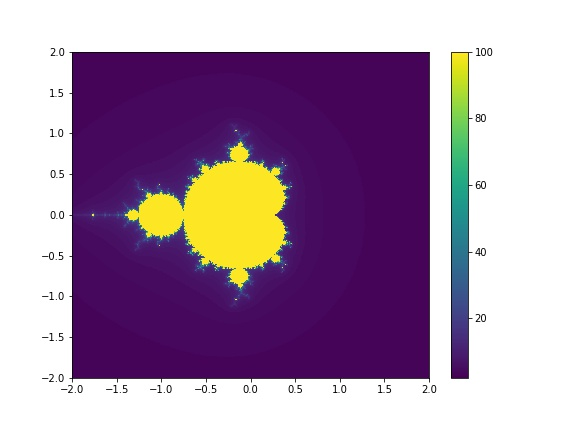
\includegraphics[width=\linewidth]{images/mandel2.jpg}
    \end{subfigure}
    \captionsetup{justification=centering,margin=1cm}
    \caption{}
    \label{fig:B0353+52}
\end{figure*}

\pagebreak

\section{Q2. Epidemics}

\subsection{Methods}

To model our epidemic, we initialize a population of 1000 residents with one preliminarily infected patient. We use a simple SIR model which keeps track of those who are Susceptible to illness (Healthy), Infected, and Recovered (or Removed from the Infected population). These three populations change with respect to he following differential equations:

\begin{align}
    \frac{dS}{dt} &= -\frac{\beta S I}{N} \\
    \frac{dI}{dt} &= \frac{\beta S I}{N} - \gamma I \\
    \frac{dR}{dt} &= \gamma I
\end{align}

$\gamma$ and $\beta$ are parameters that determine the progression of the disease. $\gamma$ represents how quickly the infected patients will recover, while $\beta$ describes the rate at which the disease spreads from the sick to the healthy. To implement this in python, a function was created which takes an array of times, initial values for S, I and R, as well as the parameters $\beta$ and $\gamma$. Using {\tt odeint} from the {\tt scipy} package, the equations were integrated over the time interval to show the following figures. In Figure \ref{fig:D}, the differential equations were modified to account for deaths related to the disease. Deceased patients are removed from the Infected population with respect to another parameter $\alpha$ as:

\begin{align}
    \frac{dS}{dt} &= -\frac{\beta S I}{N} \\
    \frac{dI}{dt} &= \frac{\beta S I}{N} - \gamma I  - \alpha D \\
    \frac{dR}{dt} &= \gamma I \\
    \frac{dD}{dt} &= \alpha D
\end{align}

In this SIRD model, we add in an initial value for D as well as the parameter $\alpha$, then integrate using the same method as above.

\subsection{Analysis}



\begin{figure}[H]
    \centering
    \captionsetup{justification=centering}
    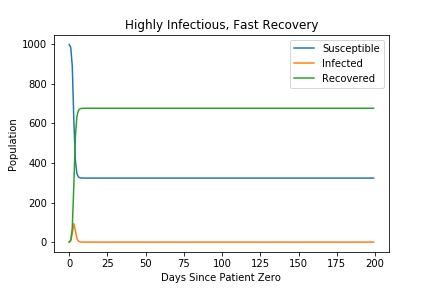
\includegraphics[width=0.8\linewidth]{images/HF.png}
    \caption{Even though the Susceptible population is quickly infected, the very fast recovery rate stamps out the infection before it can reach the majority of the population.}
    \label{fig:HF}
\end{figure}
\begin{figure}[H]
    \centering
    \captionsetup{justification=centering}
    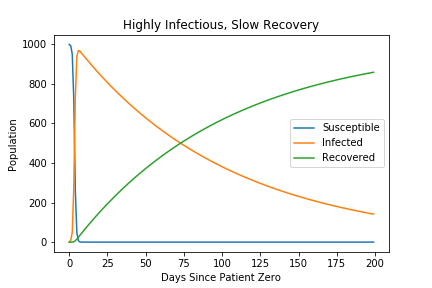
\includegraphics[width=0.8\linewidth]{images/HH.png}
    \caption{The disease quickly infects the vast majority of the population and then folks slowly recover due to the slow recovery rate. When all is said and done, this may come closer to modelling the spread of COVID-19 through countries such as the US and Italy.}
    \label{fig:HH}
\end{figure}
\begin{figure}[H]
    \centering
    \captionsetup{justification=centering}
    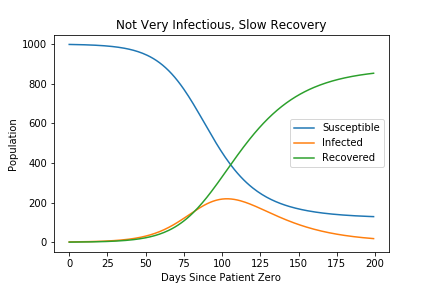
\includegraphics[width=0.8\linewidth]{images/Ns.png}
    \caption{The disease spreads slowly, physically this might reflect the effects of social distancing or just a weakly interacting virus, and not much of the population is infected. Then, with a similarly slow recovery rate, the population eventually heals without everyone incurring the disease.}
    \label{fig:Ns}
\end{figure}
\begin{figure}[H]
    \centering
    \captionsetup{justification=centering}
    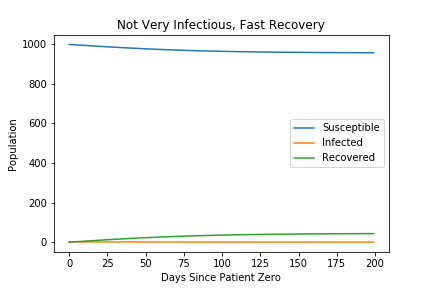
\includegraphics[width=0.8\linewidth]{images/NF.png}
    \caption{This disease has a hard time spreading from person to person, but recoveries happen rapidly, allowing most of the population to avoid ever coming in contact with the disease.}
    \label{fig:NF}
\end{figure}
\begin{figure}[H]
    \centering
    \captionsetup{justification=centering}
    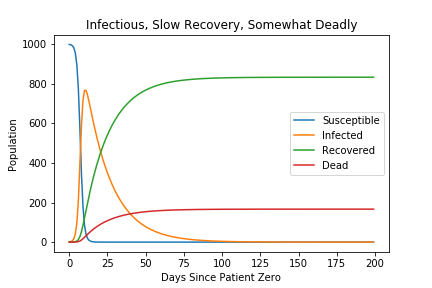
\includegraphics[width=0.8\linewidth]{images/withD.png}
    \caption{This disease will quickly infect the population while the recovery rate will have people healing fairly slowly. However, the death rate removes about 20\% of the population before they can recover.}
    \label{fig:D}
\end{figure}

\end{document}
